\section{Liên trường  - Hải Phòng- Lần 1 NH: 25--26}
\vspace{-0.5cm}
\Opensolutionfile{ans}[ans/ans-16-26-2-HaiPhong-LienTruong-L1]
\caulc
\begin{ex}%[Khanh Lê, Dự án DeTHPT 2025 - 2026]%[2H2H2-2]
Trong không gian với hệ tọa độ $Oxyz$, cho ba điểm không thẳng hàng $A(-12;10;-2)$, $B(-4;6;9)$ và $E(6;-6;4)$. Để tứ giác $ABEF$ là hình bình hành thì toạ độ điểm $F$ là
\choice
{$(-14;10;-15)$}
{$(-10;10;11)$}
{$(-22;22;3)$}
{\True $(-2;-2;-7)$}
\loigiai{
Ta có $\overrightarrow{AB}=(-4-(-12);6-10;9-(-2))=(8;-4;11)$.\\
Gọi tọa độ điểm $F$ là $(x;y;z)$. Khi đó vectơ $\overrightarrow{FE}$ là $\overrightarrow{FE}=(6-x;-6-y;4-z)$.\\
Để tứ giác $ABEF$ là hình bình hành thì ta phải có $\overrightarrow{AB}=\overrightarrow{FE}$\\
$\Rightarrow\heva{&8=6-x\\ & -4=-6-y\\ & 11=4-z}\Leftrightarrow\heva{& x=6-8\\ &  y=-6+4\\ &  z=4-11}\Leftrightarrow\heva{& x=-2\\ &  y=-2\\ &  z=-7}$.\\
Vậy tọa độ điểm $F$ là $(-2;-2;-7)$.
}
\end{ex}
\begin{ex}%[Khanh Lê, Dự án DeTHPT 2025 - 2026]%[2D1H5-1]
\immini
{
Đồ thị có hình vẽ dưới đây là của đồ thị hàm số nào?
\choice
{$y=\dfrac{-x+2}{x+1}$}
{$y=\dfrac{-x}{x+1}$}
{\True $y=\dfrac{-x+1}{x+1}$}
{$y=\dfrac{-2x+1}{2x+1}$}
}
{
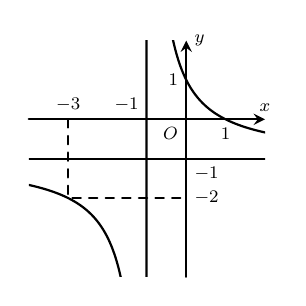
\begin{tikzpicture}[thick,scale=0.5,font=\footnotesize,line join = round, line cap = round,>=stealth]
\tikzset{every node/.style={scale=0.8}}
\draw[->] (-4,0)--(2,0)node[above]{$x$};
\draw[->] (0,-4)--(0,2)node[right]{$y$};
\draw[dashed] (-3,0)node[above]{$-3$}|-(0,-2)node[right]{$-2$};
\path (1,0)node[below]{$1$} (0,1)node[left]{$1$} (0,-1)node[below right]{$-1$} (-1,0)node[above left]{$-1$};
\fill (0,0)node[below left]{$O$};
\clip (-4,-4)rectangle(2,2);
\draw[black,samples=300,smooth] plot(\x,{(-\x+1)/(\x+1)});
\draw (-4,-1)--(2,-1);
\end{tikzpicture}
}
\loigiai{
Dựa vào đồ thị hàm số, ta phân tích các đặc điểm sau:
\begin{itemize}
\item Đồ thị nhận đường thẳng $x=-1$ làm tiệm cận đứng.
\item Đồ thị nhận đường thẳng $y=-1$ làm tiệm cận ngang.
\item Đồ thị cắt $Ox,Oy$ lần lượt tại $(1;0)$ và $(0;1)$.
\end{itemize}
}
\end{ex}
\begin{ex}%[Khanh Lê, Dự án DeTHPT 2025 - 2026]%[1D2N3-2]
Công bội của cấp số nhân $(u_n)$ biết $u_3=4$ và $u_4=8$ là
\choice
{$q=-4$}
{\True $q=2$}
{$q=\dfrac{1}{2}$}
{$q=4$}
\loigiai{
$u_{n+1}=u_n\cdot q\Rightarrow q=\dfrac{u_{n+1}}{u_n}$ $\Rightarrow q=\dfrac{u_4}{u_3}=\dfrac{8}{4}=2$.
}
\end{ex}
\begin{ex}%[Khanh Lê, Dự án DeTHPT 2025 - 2026]%[1D6H4-3]
Tập nghiệm của bất phương trình $\log_{0{,}5}(x-1)>1$ là
\choice
{$\left(-\infty;-\dfrac{3}{2}\right)$}
{$\left[1;\dfrac{3}{2}\right)$}
{\True $\left(1;\dfrac{3}{2}\right)$}
{$\left(\dfrac{3}{2};+\infty\right)$}
\loigiai{
Điều kiện xác định: $x-1>0\Leftrightarrow x>1$.\\
Ta có $\log_{0{,}5}(x-1)>1\Leftrightarrow x-1<(0{,}5)^1\Leftrightarrow x-1<0{,}5\Leftrightarrow x<1+0{,}5\Leftrightarrow x<\dfrac{3}{2}$.\\
Kết hợp nghiệm vừa tìm được với điều kiện xác định ($x>1$):
$\heva{& x>1\\ &  x<\dfrac{3}{2}}\Leftrightarrow 1<x<\dfrac{3}{2}$.\\
Vậy tập nghiệm của bất phương trình là khoảng $\left(1;\dfrac{3}{2}\right)$.
}
\end{ex}
\begin{ex}%[Khanh Lê, Dự án DeTHPT 2025 - 2026]%[2D1N3-1]
\immini
{
Cho hàm số $y=f(x)$ có đồ thị như hình bên. Hàm số đã cho đạt giá trị nhỏ nhất trên đoạn $[-1;1]$ tại
\choice
{\True $x=-1$}
{$x=0$}
{$x=-4$}
{$x=1$}
}
{
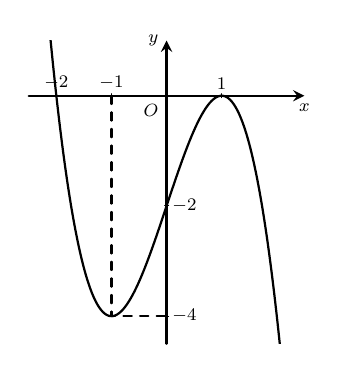
\begin{tikzpicture}[thick,scale=0.7,font=\footnotesize,line join = round, line cap = round,>=stealth]
\tikzset{every node/.style={scale=0.8}}
\draw[->] (-2.5,0)--(2.5,0)node[below]{$x$};
\draw[->] (0,-4.5)--(0,1)node[left]{$y$};
\draw[dashed] (-1,0)|-(0,-4);
\foreach \x in {-2,-1,1} \draw[thin] (\x,1pt)--(\x,-1pt) node[above]{$\x$};
\foreach \y in {-4,-2} \draw[thin] (1pt,\y)--(-1pt,\y) node[right]{$\y$};
\fill (0,0)node[below left]{$O$};
\clip (-2.5,-4.5)rectangle(2.5,1);
\draw[black,samples=300,smooth] plot(\x,{-\x^3+3*\x-2});
\end{tikzpicture}
}
\loigiai{
Dựa vào đồ thị ta thấy hàm số đã cho đạt giá trị nhỏ nhất trên đoạn $[-1;1]$ tại điểm $x=-1$.
}
\end{ex}
\begin{ex}%[Khanh Lê, Dự án DeTHPT 2025 - 2026]%[1H8H6-2]
	Cho hình chóp $S.ABC$ có $SA\perp(ABC)$, $SA=\dfrac{3a}{2}$, đáy $ABC$ là tam giác đều cạnh $a$. Tính số đo của góc nhị diện $[S,BC,A]$.
	\choice
	{$30^\circ$}
	{$90^\circ$}
	{$120^\circ$}
	{\True $60^\circ$}
	\loigiai{
		\begin{center}
			\begin{tikzpicture}[thick,scale=1, font=\footnotesize,line join=round, line cap=round, >=stealth]
				\def\h{3}
				\path (0,0)coordinate(A)--(4,0)coordinate(C)--(1.5,-1.5)coordinate(B)--($(A)+(0,\h)$)coordinate(S);
				\coordinate (M) at ($(C)!0.5!(B)$);
				\draw (S)--(A)--(B)--(C)--cycle (S)--(B) (S)--(M);
				\draw[dashed] (A)--(C) (A)--(M);
				\path pic[draw,angle radius=5]{right angle=A--M--B};
				\path pic[draw,angle radius=5]{right angle=S--M--C};
				\path pic[draw,blue,angle radius=15,angle eccentricity=1.5,"$\varphi$"]{angle=S--M--A};
				\foreach \x/\g in {S/90,A/150,C/30,B/-90,M/-30}\fill (\x) circle (1pt)+(\g:0.25)node{$\x$};
			\end{tikzpicture}
		\end{center}
		Gọi $M$ là trung điểm $BC$.\\
		Vì tam giác $ABC$ đều cạnh $a$ nên $AM\perp BC$\quad(1) và $AM=\dfrac{a\sqrt{3}}{2}$.\\
		Lại có $SA\perp(ABC)$ nên $SA\perp BC$, từ đó suy ra $SM\perp BC$.\quad(2)\\
		Từ (1) và (2) ta có $[S,BC,A]=\widehat{SMA}$.\\
		Tam giác $SAM$ vuông tại $A$, nên $\tan\widehat{SMA}=\dfrac{SA}{AM}=\dfrac{\dfrac{3a}{2}}{\dfrac{a\sqrt{3}}{2}}=\sqrt{3}\Rightarrow\widehat{SMA}=60^\circ$.
	}
\end{ex}
\begin{ex}%[Khanh Lê, Dự án DeTHPT 2025 - 2026]%[2D1H4-1]
Cho hàm số $y=f(x)$ có bảng biến thiên như hình bên dưới.
\begin{center}

\begin{tikzpicture}[thick]
\tkzTabInit[nocadre,lgt=1.2,espcl=2.5,deltacl=0.6]
{$x$/.6,$y'$/.6,$y$/2}
{$-\infty$,$1$,$3$,$+\infty$}
\tkzTabLine{,+,d,+,0,-,}
\tkzTabVar{-/$-1$,+D-/$+\infty$/$-\infty$,+/$2$,-/$-\infty$}
\end{tikzpicture}
\end{center}
Đồ thị hàm số $y=f(x)$ có tổng số bao nhiêu đường tiệm cận đứng và ngang?
\choice
{\True $2$}
{$0$}
{$1$}
{$3$}
\loigiai{
Từ bảng biến thiên, ta có $\lim\limits_{x\to 1^+}f(x)=-\infty$ nên đồ thị hàm số có đường tiệm cận đứng là $x=1$.\\
Và $\lim\limits_{x\to-\infty}f(x)=-1$ nên đồ thị hàm số có đường tiệm cận ngang là $y=-1$.\\
Vậy đồ thị hàm số $y=f(x)$ có tổng cộng $2$ đường tiệm cận đứng và ngang.
}
\end{ex}
\begin{ex}%[Khanh Lê, Dự án DeTHPT 2025 - 2026]%[1D9H1-3]
Hai khẩu pháo cao xạ cùng bắn độc lập với nhau vào một mục tiêu. Xác suất bắn trúng mục tiêu của hai khẩu pháo cao xạ lần lượt là $\dfrac{1}{4}$ và $\dfrac{1}{3}$. Xác suất để mục tiêu bị bắn trúng đạn là
\choice
{\True $\dfrac{1}{2}$}
{$\dfrac{7}{12}$}
{$\dfrac{5}{12}$}
{$\dfrac{1}{4}$}
\loigiai{
Gọi $A$: \lq\lq Xạ thủ 1 bắn trúng mục tiêu\rq\rq.\\
$B$: \lq\lq Xạ thủ 2 bắn trúng mục tiêu\rq\rq.\\
$M$: \lq\lq Mục tiêu bị bắn trúng\rq\rq.\\
Theo giả thiết ta có: $\mathrm{P}(A)=\dfrac{1}{4}\Rightarrow \mathrm{P}(\overline{A})=1-\dfrac{1}{4}=\dfrac{3}{4}$.\\
Và $\mathrm{P}(B)=\dfrac{1}{3}\Rightarrow \mathrm{P}(\overline{B})=1-\dfrac{1}{3}=\dfrac{2}{3}$.\\
Ta có $\overline{M}=\overline{A}\cap \overline{B}$. Vì $A$ và $B$ là hai biến cố độc lập nên $\overline{A}$ và $\overline{B}$ cũng là hai biến cố độc lập.\\
Do đó $\mathrm{P}(\overline{M})=\mathrm{P}(\overline{A})\cdot \mathrm{P}(\overline{B})=\dfrac{3}{4}\cdot \dfrac{2}{3}=\dfrac{1}{2}$.\\
Vậy $\mathrm{P}(M)=1-\mathrm{P}(\overline{M})=\dfrac{1}{2}$.
}
\end{ex}
\begin{ex}%[Khanh Lê, Dự án DeTHPT 2025 - 2026]%[1D1N5-3]
Phương trình $\sin x=-1$ có nghiệm là
\choice
{$x=\dfrac{\pi}{2}+k 2\pi,k\in\mathbb{Z}$}
{$x=\pi+k 2\pi,k\in\mathbb{Z}$}
{$x=k\pi,k\in\mathbb{Z}$}
{\True $x=-\dfrac{\pi}{2}+k 2\pi,k\in\mathbb{Z}$}
\loigiai{
Ta có $\sin x=-1\Leftrightarrow x=-\dfrac{\pi}{2}+k 2\pi,k\in\mathbb{Z}$.
}
\end{ex}
\begin{ex}%[Khanh Lê, Dự án DeTHPT 2025 - 2026]%[1D5H1-3]
Khảo sát thu nhập theo tháng của người lao động ở một công ty thu được mẫu số liệu ghép nhóm như sau
\begin{center}
\begin{tabular}{|c|c|c|c|c|c|}
\hline
Thu nhập (triệu đồng )&$[5;8)$&$[8;11)$&$[11;14)$&$[14;17)$&$[17;20)$\\
\hline
Số người&30&55&45&30&20\\
\hline
\end{tabular}
\end{center}
Tính thu nhập trung bình của người lao động công ty?
\choice
{$10{,}5$}
{\True $11{,}75$}
{$12{,}5$}
{$11$}
\loigiai{
\begin{center}
\begin{tabular}{|c|c|c|c|c|c|}
\hline
Thu nhập (triệu đồng )&$[5;8)$&$[8;11)$&$[11;14)$&$[14;17)$&$[17;20)$\\
\hline
Số người&30&55&45&30&20\\
\hline
Giá trị đại diện&$6{,}5$&$9{,}5$&$12{,}5$&$15{,}5$&$18{,}5$\\
\hline
\end{tabular}
\end{center}
Thu nhập trung bình của người lao động công ty là
\[\overline{x}=\dfrac{6{,}5\cdot 30+9{,}5\cdot 55+12{,}5\cdot 45+15{,}5\cdot 30+18{,}5\cdot 20}{30+55+45+30+20}\approx 11{,}75.\]
}
\end{ex}
\begin{ex}%[Khanh Lê, Dự án DeTHPT 2025 - 2026]%[2D1N2-2]
Cho hàm số $y=f(x)$ có bảng biến thiên như sau:
\begin{center}

\begin{tikzpicture}[thick]
\tkzTabInit[nocadre,lgt=1.2,espcl=2.5,deltacl=0.6]
{$x$/.6,$y'$/.6,$y$/2}
{$-\infty$,$0$,$3$,$+\infty$}
\tkzTabLine{,+,0,-,0,+,}
\tkzTabVar{-/$-\infty$,+/$2$,-/$-4$,+/$+\infty$}
\end{tikzpicture}
\end{center}
Hàm số $f(x)$ đạt cực tiểu tại điểm
\choice
{$y=0$}
{$x=-4$}
{$y=-4$}
{\True $x=3$}
\loigiai{
Từ BBT ta thấy hàm số $f(x)$ đạt cực tiểu tại điểm $x=3$.
}
\end{ex}
\begin{ex}%[Khanh Lê, Dự án DeTHPT 2025 - 2026]%[2H2N2-2]
Trong không gian $Oxyz$, cho điểm $A(1;0;1)$. Tìm tọa độ điểm $C$ thỏa mãn $\overrightarrow{AC}=(3;3;0)$?
\choice
{$C(2;3;1)$}
{$C(3;3;0)$}
{$C(-3;-3;-1)$}
{\True $C(4;3;1)$}
\loigiai{
Giả sử $C(x;y;z)$ $\Rightarrow\overrightarrow{AC}=(x-1;y;z-1)$.\\
Do đó: $\overrightarrow{AC}=(3;3;0)\Leftrightarrow\heva{ & x-1=3\\ & y=3\\ & z-1=0}\Leftrightarrow\heva{ & x=4\\ & y=3\\ & z=1}$.\\
Vậy $C(4;3;1)$.
}
\end{ex}


\Closesolutionfile{ans}

\cauds
\Opensolutionfile{ans}[ans/ans-16-26-2-HaiPhong-LienTruong-L1-DS]
\begin{ex}%[Khanh Lê, Dự án DeTHPT 2025 - 2026]%[2H5V2-7]
Cho hình vuông $ABCD$ có cạnh bằng $4$. Lấy $H$, $K$ lần lượt trên các cạnh $AB$, $AD$ sao cho $BH=3HA$, $AK=3KD$. Trên đường thẳng vuông góc với mặt phẳng $(ABCD)$ tại $H$ lấy điểm $S$ sao cho $\widehat{SBH}=30^\circ$.
\choiceTF
{Thể tích của khối chóp $S.ABC$ bằng $\dfrac{16\sqrt{3}}{3}$}
{\True Khoảng cách giữa $AB$ và $SD$ bằng $\dfrac{4\sqrt{57}}{19}$}
{\True $SH=\sqrt{3}$}
{\True Gọi $E$ là giao điểm của $CH$ và $BK$, côsin của góc giữa hai đường thẳng $SE$ và $BC$ bằng $\dfrac{m}{n\sqrt{39}}$ với $m\in\mathbb{Z}$; $n\in\mathbb{N}^*$; $\dfrac{m}{n}$ là phân số tối giản. Giá trị của biểu thức $T=2m-n=31$}
\loigiai{
\begin{center}
\begin{tikzpicture}[thick,scale=1, font=\footnotesize,line join=round, line cap=round, >=stealth]
\def\h{3}
\path (0,0)coordinate(A)--(3.5,0)coordinate(D)--(220:2.5)coordinate(B)--($(B)+(D)-(A)$)coordinate(C)--($(A)!0.25!(B)$)coordinate(H)--($(H)+(0,\h)$)coordinate(S);
\coordinate (F) at ($(D)!0.25!(C)$);
\coordinate (K) at ($(A)!0.75!(D)$);
\coordinate (E) at (intersection of H--C and B--K);
\coordinate (N) at ($(S)!0.7!(F)$);
\draw (S)--(D)--(C)--(B)--cycle (S)--(C) (S)--(F);
\draw[dashed] (S)--(A)--(D) (A)--(B) (S)--(H)--(C) (B)--(K) (S)--(E) (N)--(H)--(F);
\draw[->](S)--++(90:0.5)node[right]{$z$};
\draw[->](B)--++(220:0.5)node[above]{$x$};
\draw[->](F)--++(0:0.5)node[below]{$y$};
\foreach \x/\g in {S/150,A/150,D/30,C/-90,B/-90,H/180,K/60,E/-90,F/-80,N/20}\fill (\x) circle (1pt)+(\g:0.25)node{$\x$};
\path pic[draw,angle radius=5]{right angle=S--H--A};
\path pic[draw,angle radius=5]{right angle=H--N--S};
\path pic[draw,blue,angle radius=15,angle eccentricity=1.5,"\tiny $30^\circ$"]{angle=H--B--S};
\end{tikzpicture}
\end{center}
\begin{itemchoice}
\itemch Ta có $V_{S.ABCD}=\dfrac{1}{3}SH\cdot S_{ABCD}$.\\
$S_{ABCD}=4^2=16$, $HB=\dfrac{3}{4}AB=3$, $\tan 30^\circ=\dfrac{SH}{HB}\Rightarrow SH=3\cdot \tan 30^\circ=\sqrt{3}$.\\
Suy ra $V_{S.ABCD}=\dfrac{1}{3}\cdot \sqrt{3}\cdot 16=\dfrac{16\sqrt{3}}{3}$ mà $V_{S.ABC}=\dfrac{1}{2}V_{S.ABCD}=\dfrac{8\sqrt{3}}{3}$.
\itemch Dựng $HF\perp CD$ tại $F$ và $HN\perp SF$ tại $N$.\\
Ta có $AB\parallel (SCD)$ nên $\mathrm{d}(AB,SD)=\mathrm{d}(AB,(SCD))=\mathrm{d}(H,(SCD))=HN$.\\
Xét tam giác $SHF$ vuông tại $H$ có: \[\dfrac{1}{HS^2}+\dfrac{1}{HF^2}=\dfrac{1}{HN^2}\Leftrightarrow\dfrac{1}{(\sqrt{3})^2}+\dfrac{1}{4^2}=\dfrac{1}{HN^2}\Rightarrow HN=\dfrac{4\sqrt{57}}{19}.\]
Vậy $\mathrm{d}(AB,SD)=\dfrac{4\sqrt{57}}{19}$.
\itemch Ta có $SH=HB\cdot\tan\widehat{SBH}=3\cdot\tan 30^\circ=\sqrt{3}$.
\itemch Đặt hệ trục $Oxyz$ như hình trên.\\
$H(0;0;0)$, $S(0;0;\sqrt{3})$, $B(3;0;0)$, $C(3;4;0)$, $K(-1;3;0)$.\\
Mà $E=CH\cap  BK$ với $CH\colon \heva{ & x=3t\\ & y=4t\\ & z=0}$ và $BK\colon \heva{ & x=3-4t'\\ & y=3t'\\ & z=0}$
nên $\heva{ &3t=3-4t'\\ &4t=3t'}\Leftrightarrow\heva{ & t=\dfrac{9}{25}\\ & t'=\dfrac{12}{25}}$.\\
Suy ra $E\left(\dfrac{27}{25};\dfrac{36}{25};0\right)\Rightarrow\overrightarrow{SE}=\left(\dfrac{27}{25};\dfrac{36}{25};-\sqrt{3}\right)$; $\overrightarrow{BC}=(0;4;0)$.\\
$\cos(SE,BC)=|\cos(\overrightarrow{SE},\overrightarrow{BC})|=\dfrac{|\overrightarrow{SE}\cdot \overrightarrow{BC}|}{|\overrightarrow{SE}||\overrightarrow{BC}|}=\dfrac{\dfrac{144}{25}}{\dfrac{2\sqrt{39}}{5}\cdot 4}=\dfrac{18}{5\sqrt{39}}\Rightarrow\heva{ & m=18\\ & n=5}$.\\
Vậy $T=2m-n=2\cdot 18-5=31$.
\end{itemchoice}
}
\end{ex}
\begin{ex}%[Khanh Lê, Dự án DeTHPT 2025 - 2026]%[2H5H3-4]
Trong không gian, xét hệ toạ độ $Oxyz$ có gốc $O$ trùng với vị trí một giàn khoan trên biển, mặt phẳng $(Oxy)$ trùng với mặt biển (được gọi là mặt phẳng) với tia $Ox$ hướng về phía nam, tia $Oy$ hướng về phía đông, tia $Oz$ hướng thẳng lên trời (tham khảo hình vẽ). Đơn vị đo trong không gian $Oxyz$ lấy theo kilômét. Một chiếc radar đặt tại $O$ có phạm vi theo dõi $30$ km. Một chiếc tàu thám hiểm tại vị trí $A$ ở độ sâu $10$ km so với mặt nước biển, cách $O$ $25$ km về phía nam và $15$ km về phía tây. Một tàu đánh cá tại vị trí $B(-20;15;0)$.
\choiceTF
{\True Một chiếc tàu của cảnh sát biển đang tuần tra di chuyển đến vị trí $C$ cách $O$ $15$ km về phía nam. Để radar phát hiện ra thì tàu cảnh sát biển cần di chuyển về phía đông cách $O$ tối đa $15\sqrt{3}$ km}
{\True Radar phát hiện ra tàu đánh cá tại vị trí $B$}
{\True Khoảng cách từ chiếc tàu thám hiểm đến radar bằng $3\sqrt{58}$ km}
{\True Radar không phát hiện được tàu thám hiểm đặt tại vị trí $A$}
\loigiai{
\begin{itemchoice}
\itemch Gọi $x$(km), $x>0$ là khoảng cách từ tàu cảnh sát biển cách radar $O$ về phía đông. Khi đó toạ độ của tàu cảnh sát biển là $C(15;x;0)$.\\
Ta có $OC=\sqrt{15^2+x^2+0^2}=\sqrt{x^2+225}$.\\
Để radar phát hiện được tàu cảnh sát biển thì $OC\le 30$ km.\\
Suy ra $\sqrt{x^2+225}\le 30\Leftrightarrow x^2+225\le 900\Leftrightarrow x^2\le 675\Leftrightarrow x\le 15\sqrt{3} $ km.\\
Vậy tàu cảnh sát biển cần di chuyển về phía đông cách $O$ tối đa $15\sqrt{3}$ km.
\itemch Ta có $OB=\sqrt{(-20)^2+15^2+0^2}=25<30$ km nên radar phát hiện ra tàu đánh cá tại vị trí $B$.
\itemch Một chiếc tàu thám hiểm tại vị trí $A$ ở độ sâu $10$ km so với mặt nước biển, cách $O$ $25$ km về phía nam và $15$ km về phía tây nên ta có toạ độ tàu thám hiểm là điểm toạ độ điểm $A(25;-15;-10)$. Khi đó khoảng cách từ chiếc tàu thám hiểm đến radar bằng \[OA=\sqrt{25^2+(-15)^2+(-10)^2}=5\sqrt{38}\text{ km}.\]
\itemch Ta thấy $OA=5\sqrt{38}\approx 30{,}82$ km, mà phạm vi theo dõi của radar là $30$ km nên radar không phát hiện được tàu thám hiểm đặt tại vị trí $A$.
\end{itemchoice}
}
\end{ex}
\begin{ex}%[Khanh Lê, Dự án DeTHPT 2025 - 2026]%[2D1H5-7]
Cho hàm số $f(x)=\dfrac{2x^2-5x+9}{x-5}$. Khi đó:
\choiceTF
{\True Đồ thị hàm số cắt trục tung tại điểm có tung độ bằng $-\dfrac{9}{5}$}
{Hàm số nghịch biến trên khoảng $(1;9)$}
{Có đúng một điểm trên đồ thị cách đều hai trục tọa độ}
{Đồ thị hàm số có tiệm cận đứng là $y=5$}
\loigiai{
\begin{itemchoice}
\itemch Với $x=0\Rightarrow f(0)=-\dfrac{9}{5}$.\\
Vậy đồ thị hàm số cắt trục tung tại điểm có tung độ bằng $-\dfrac{9}{5}$.
\itemch Tập xác định của hàm số là $\mathbb{R}\setminus\{5\}$ suy ra hàm số đã cho không xác định $\forall x\in(1;9)$. Do đó hàm số không nghịch biến trên khoảng $(1;9)$.
\itemch Gọi $M(x_0;y_0)$ thuộc đồ thị hàm số (điều kiện $x_0\ne 5$).\\
Vì điểm $M(x_0;y_0)$ trên đồ thị cách đều hai trục tọa độ nên $y_0=\pm x_0$.
\begin{itemize}
\item TH1: $y_0=x_0$
$\Leftrightarrow\dfrac{2x_0^2-5x_0+9}{x_0-5}=x_0\Leftrightarrow 2x_0^2-5x_0+9=x_0^2-5x_0\Leftrightarrow x_0^2+9=0$ (phương trình vô nghiệm).
\item TH2: $y_0=-x_0$
$\Leftrightarrow\dfrac{2x_0^2-5x_0+9}{x_0-5}=-x_0\Leftrightarrow 2x_0^2-5x_0+9=-x_0^2+5x_0$
$\Leftrightarrow 3x_0^2-10x_0+9=0$ (phương trình vô nghiệm).
\end{itemize}
Vậy không có điểm nào trên đồ thị cách đều hai trục tọa độ.
\itemch Ta có $\lim\limits_{x \to 5^+}f(x)=+\infty$. Đồ thị hàm số có tiệm cận đứng là $x=5$.
\end{itemchoice}
}
\end{ex}
\begin{ex}%[Khanh Lê, Dự án DeTHPT 2025 - 2026]%[1D1V5-3]
Cho phương trình $\cos\left(4x-\dfrac{3\pi}{8}\right)=-1$. Khi đó:
\choiceTF
{\True $x=\dfrac{11\pi}{32}$ là một nghiệm của phương trình đã cho}
{\True Tất cả nghiệm của phương trình đã cho được biểu diễn bởi 4 điểm trên đường tròn lượng giác}
{Tổng nghiệm dương nhỏ nhất và nghiệm âm lớn nhất của phương trình bằng $\dfrac{3\pi}{4}$}
{Tổng các nghiệm trên khoảng $\left(\dfrac{\pi}{4};\dfrac{19\pi}{2}\right)$ của phương trình đã cho là $\dfrac{6061\pi}{32}$}
\loigiai{
\begin{itemchoice}
\itemch Thay $x=\dfrac{11\pi}{32}$ vào phương trình, ta được: $\cos\left(4\cdot \dfrac{11\pi}{32}-\dfrac{3\pi}{8}\right)=\cos\left(\pi\right)=-1$.\\
Vậy $x=\dfrac{11\pi}{32}$ là một nghiệm của phương trình đã cho.
\itemch Ta có: $\cos\left(4x-\dfrac{3\pi}{8}\right)=-1$$\Leftrightarrow 4x-\dfrac{3\pi}{8}=\pi+k 2\pi$$\Leftrightarrow 4x=\dfrac{11\pi}{8}+k 2\pi$$\Leftrightarrow x=\dfrac{11\pi}{32}+\dfrac{k\pi}{2}(k\in\mathbb{Z})$.\\
Áp dụng công thức nghiệm: $x=\alpha+\dfrac{k 2\pi}{n}$ với $n$ là số điểm biểu diễn trên đường tròn lượng giác, ta có: $\Leftrightarrow x=\dfrac{11\pi}{32}+\dfrac{k\pi}{2}=\dfrac{11\pi}{32}+\dfrac{k 2\pi}{4}$. Suy ra $n=4$.\\
Vậy tất cả nghiệm của phương trình đã cho được biểu diễn bởi 4 điểm trên đường tròn lượng giác.
\itemch Xét $x=\dfrac{11\pi}{32}+\dfrac{k\pi}{2}>0$$\Leftrightarrow\dfrac{k\pi}{2}>-\dfrac{11\pi}{32}$$\Leftrightarrow k>-\dfrac{11}{16}$ mà $k\in\mathbb{Z}\Rightarrow$ nghiệm dương nhỏ nhất ứng với $k=0$.\\
Nghiệm dương nhỏ nhất là $\dfrac{11\pi}{32}+\dfrac{0\cdot \pi}{2}=\dfrac{11\pi}{32}$.\\
Xét $x=\dfrac{11\pi}{32}+\dfrac{k\pi}{2}<0$$\Leftrightarrow\dfrac{k\pi}{2}<-\dfrac{11\pi}{32}$$\Leftrightarrow k<-\dfrac{11}{16}$ mà $k\in\mathbb{Z}\Rightarrow$ nghiệm âm lớn nhất ứng với $k=-1$.\\
Nghiệm âm lớn nhất là $\dfrac{11\pi}{32}+\dfrac{(-1)\cdot \pi}{2}=-\dfrac{5\pi}{32}$.\\
Tổng nghiệm dương nhỏ nhất và nghiệm âm lớn nhất của phương trình bằng $\dfrac{11\pi}{32}-\dfrac{5\pi}{32}=\dfrac{3\pi}{16}$.
\itemch Ta có
\allowdisplaybreaks
\begin{eqnarray*}
x\in\left(\dfrac{\pi}{4};\dfrac{19\pi}{2}\right)&\Leftrightarrow&\dfrac{\pi}{4}<x<\dfrac{19\pi}{2}\\
&\Leftrightarrow&\dfrac{\pi}{4}<\dfrac{11\pi}{32}+\dfrac{k\pi}{2}<\dfrac{19\pi}{2}\\
&\Leftrightarrow&\dfrac{1}{4}<\dfrac{11}{32}+\dfrac{k}{2}<\dfrac{19}{2}\\
&\Leftrightarrow&-\dfrac{3}{32}<\dfrac{k}{2}<\dfrac{293}{32}\\
&\Leftrightarrow&-\dfrac{3}{16}<k<\dfrac{293}{16},k\in\mathbb{Z}\\
&\Rightarrow& k\in\{0;1;2;\ldots;17;18\}
\end{eqnarray*}
Thay các giá trị của $k$ vào $x=\dfrac{11\pi}{32}+\dfrac{k\pi}{2}$ ta được tập hợp các nghiệm trên khoảng $\left(\dfrac{\pi}{4};\dfrac{19\pi}{2}\right)$: $x\in\left\{\dfrac{11\pi}{32};\dfrac{11\pi}{32}+\dfrac{\pi}{2};\dfrac{11\pi}{32}+\dfrac{2\pi}{2};\ldots;\dfrac{11\pi}{32}+\dfrac{17\pi}{2};\dfrac{11\pi}{32}+\dfrac{18\pi}{2}\right\}$.\\
Tính tổng các nghiệm có 2 cách:
\begin{itemize}
\item Cách 1: Bấm máy $\sum\limits_{k=0}^{18}\left(\dfrac{11\pi}{32}+\dfrac{k\pi}{2}\right)=\dfrac{2945\pi}{32}$.
\item Cách 2: Tính: $\dfrac{11\pi}{32}+\left(\dfrac{11\pi}{32}+\dfrac{\pi}{2}\right)+\left(\dfrac{11\pi}{32}+\dfrac{2\pi}{2}\right)+\cdots+\left(\dfrac{11\pi}{32}+\dfrac{17\pi}{2}\right)+\left(\dfrac{11\pi}{32}+\dfrac{18\pi}{2}\right)$.\\
Coi mỗi nghiệm là 1 số hạng trong cấp số cộng với $x_1=\dfrac{11\pi}{32}$, công sai $d=\dfrac{\pi}{2}$.\\
Do $k\in\{0;1;2;\ldots;17;18\}$ nên số số hạng $n=19$.\\
Tổng các nghiệm là: $S=\dfrac{\left(x_1+x_{19}\right)\cdot n}{2}=\dfrac{\left(\dfrac{11\pi}{32}+\dfrac{11\pi}{32}+\dfrac{18\pi}{2}\right)\cdot 19}{2}=\dfrac{2945\pi}{32}$.
\end{itemize}
\end{itemchoice}
}
\end{ex}


\Closesolutionfile{ans}

\Opensolutionfile{ans}[ans/ans-16-26-2-HaiPhong-LienTruong-L1-KQ]
\caukq
\begin{ex}%[Khanh Lê, Dự án DeTHPT 2025 - 2026]%[1H8V5-4]
Cho hình chóp $S.ABCD$ có đáy $ABCD$ là hình thoi cạnh $1$, góc $\widehat{BAD}=60^\circ $. Tam giác $SAB$ vuông cân tại $S$ và nằm trong mặt phẳng vuông góc với đáy. Biết khoảng cách từ $AB$ đến $SC$ bằng $\dfrac{\sqrt{a}}{b}(a;b\in\mathbb{Z}^*)$ ($\dfrac{a}{b}$ là phân số tối giản). Tính tổng $a+b$?
\shortans{$7$}
\loigiai{
\begin{center}
\begin{tikzpicture}[thick,scale=1, font=\footnotesize,line join=round, line cap=round, >=stealth]
\def\h{3}
\path (0,0)coordinate(A)--(4,0)coordinate(D)--(220:2)coordinate(B)--($(B)+(D)-(A)$)coordinate(C)--($(A)!0.5!(B)$)coordinate(I)--($(I)+(0,\h)$)coordinate(S);
\coordinate (O) at (intersection of A--C and B--D);
\coordinate (H) at ($(S)!0.6!(D)$);
\draw (S)--(D)--(C)--(B)--cycle (S)--(C);
\draw[dashed] (S)--(A)--(D) (A)--(B)--(D) (S)--(I)--(D) (A)--(C) (I)--(H);
\foreach \x/\g in {S/90,A/60,D/30,C/-90,B/-90,I/180,O/-90,H/30}\fill (\x) circle (1pt)+(\g:0.25)node{$\x$};
\path pic[draw,angle radius=5]{right angle=S--I--A};
\path pic[draw,angle radius=5]{right angle=A--O--D};
\path pic[draw,angle radius=5]{right angle=I--H--S};
\path pic[draw,angle radius=5]{right angle=B--I--D};
\path pic[draw,blue,angle radius=5,angle eccentricity=1.5,"$60^\circ$"]{angle=B--A--D};
\end{tikzpicture}
\end{center}
Vì $\widehat{BAD}=60^\circ$ nên $\triangle ABC$ là tam giác đều cạnh bằng $1$.\\
Gọi $I$ là trung điểm của $AB$.\\
$\triangle ABD$ là tam giác đều nên $DI\perp AB$.\\
Vì tam giác $SAB$ vuông cân tại $S$ và nằm trong mặt phẳng vuông góc với đáy nên $SI\perp (ABCD)$.\\
Gọi $H$ là chân đường vuông góc kẻ từ $I$ đến $SD$.\\
$\heva{ & AB\perp SI\\ & AB\perp DI}\Rightarrow AB\perp(SDI)\Rightarrow AB\perp IH$ mà $AB\parallel CD$ do đó $IH\perp CD$.\\
Lại có $IH\perp SD$ suy ra $IH\perp (SCD)$.\\
Ta có: $AB\parallel CD$ nên $AB\parallel(SCD)$.\\
Khi đó: $\mathrm{d}(AB,SC)=\mathrm{d}(AB,(SCD))=\mathrm{d}(I,(SCD))=IH$.\\
$ID=\dfrac{\sqrt{3}}{2}$ và $SI=\dfrac{1}{2}AB=\dfrac{1}{2}$ suy ra $IH=\sqrt{\dfrac{SI^2\cdot ID^2}{SI^2+ID^2}}=\sqrt{\dfrac{\left(\frac{1}{2}\right)^2\cdot \left(\frac{\sqrt{3}}{2}\right)^2}{\left(\frac{1}{2}\right)^2+\left(\frac{\sqrt{3}}{2}\right)^2}}=\dfrac{\sqrt{3}}{4}$.\\
Vậy $a=3$ và $b=4$ suy ra $a+b=7$.
}
\end{ex}
\begin{ex}%[Khanh Lê, Dự án DeTHPT 2025 - 2026]%[2D1V3-6]
Một doanh nghiệp sản xuất độc quyền một loại sản phẩm. Giả sử khi sản xuất và bán hết $x$ sản phẩm $(0<x\le 2500)$, tổng số tiền doanh nghiệp thu được là $f(x)=2006x-x^2$ (đơn vị: nghìn đồng) và tổng chi phí là $g(x)=x^2+1438x-1209$ (đơn vị: nghìn đồng). Giả sử mức thuế phụ thu trên một đơn vị sản phẩm bán được là $t$ (nghìn đồng) $(0<t<320)$. Giá trị của $t$ bằng bao nhiêu nghìn đồng để nhà nước nhận được số tiền thuế phụ thu lớn nhất và doanh nghiệp cũng nhận được lợi nhuận lớn nhất theo mức thuế phụ thu đó?
\shortans{$284$}
\loigiai{
Gọi $h(x)$ là lợi nhuận của doanh nghiệp khi bán $x$ sản phẩm với mức thuế $t$.\\
Ta có: $h(x)=f(x)-g(x)-tx=(2006x-x^2)-(x^2+1438x-1209)-tx$.\\
$\Rightarrow h(x)=-2x^2+(568-t)x+1209$ $\Rightarrow h'(x)=-4x+(568-t)=0\Rightarrow x=\dfrac{568-t}{4}$.\\
Vì $h(x)$ là hàm bậc hai có $a<0$ nên suy ra $\max h(x)=h\left(\dfrac{568-t}{4}\right)$.\\
Số tiền thuế nhà nước thu được để doanh nghiệp cũng nhận được lợi nhuận lớn nhất là $T(t)$:\\
$T(t)=tx=t\left(\dfrac{568-t}{4}\right)=\dfrac{1}{4}t(568-t)\le\dfrac{1}{4}\left(\dfrac{t+568-t}{2}\right)^2=20164$.\\
Dấu ``='' xảy ra khi $t=568-t\Leftrightarrow t=284$ (thỏa mãn điều kiện $0<t<320$).\\
Suy ra, $\max T(t)=20164$ khi $t=284$.\\
Vậy giá trị của thuế phụ thu cần tìm là $t=284$ (nghìn đồng).
}
\end{ex}
\begin{ex}%[Khanh Lê, Dự án DeTHPT 2025 - 2026]%[1D6V4-6]
Trong năm đầu tiên đi làm, anh Huy nhận được lương là 10 triệu đồng mỗi tháng. Cứ hết một năm, anh Huy lại được tăng lương, mỗi tháng năm sau tăng $12\%$ so với mỗi tháng năm trước. Kể từ năm thứ 2 mỗi khi lĩnh lương anh Huy đều cất đi phần tăng lương so với năm ngay trước để tiết kiệm mua ô tô. Hỏi tính từ khi đi làm sau ít nhất bao nhiêu năm thì anh Huy mua được ô tô giá 500 triệu biết rằng anh Huy được gia đình hỗ trợ $32\%$ giá trị chiếc xe?
\shortans{$13$}
\loigiai{
Số tiền mà anh Huy phải trả để mua xe ô tô là: $500\cdot 0{,}68=340$ (triệu đồng).\\
Tổng tiền lương năm đầu tiên: $T_1=10\cdot 12=120$ (triệu đồng).\\
Số tiền tiết kiệm được sau năm thứ hai là: $T_2=120\cdot 1{,}12-120=120\cdot 0{,}12$ (triệu đồng).\\
Số tiền tiết kiệm được sau năm thứ ba là: $T_3=120\cdot 1{,}12^2-120\cdot 1{,}12=120\cdot 1{,}12\cdot 0{,}12$ (triệu đồng).\\
\ldots\\
Số tiền tiết kiệm được sau năm thứ $n$ là: $T_n=120\cdot 1{,}12^{n-2}\cdot 0{,}12$ (triệu đồng).\\
Tổng số tiền tiết kiệm của anh Huy sau $n$ năm là:
\allowdisplaybreaks
\begin{eqnarray*}
T=T_2+T_3+\cdots+T_n&=&120\cdot 0{,}12(1+1{,}12+1{,}12^2+\cdots+1{,}12^{n-2})\\
&=&120\cdot 0{,}12\cdot \dfrac{1{,}12^{n-1}-1}{1{,}12-1}\\
&=&120\cdot (1{,}12^{n-1}-1)\text{ (triệu đồng)}.
\end{eqnarray*}
Để anh Huy đủ tiền mua xe thì:
\[T\ge 340\Rightarrow 120\cdot \left(1{,}12^{n-1}-1\right)\ge 340\Rightarrow n-1\ge\log_{1{,}12}\left(\dfrac{23}{6}\right)\Rightarrow n\ge 12{,}8.\]
Vậy tính từ khi đi làm, phải ít nhất 13 năm thì anh Huy mới đủ tiền mua ô tô.
}
\end{ex}
\begin{ex}%[Khanh Lê, Dự án DeTHPT 2025 - 2026]%[2H2V2-6]
Hai chiếc flycam được điều khiển cùng bay lên tại một địa điểm. Sau một thời gian bay, chiếc flycam thứ nhất cách điểm xuất phát về phía Bắc $20$(m) và về phía Tây $10$(m), đồng thời cách mặt đất $0{,}7$(m). chiếc flycam thứ hai cách điểm xuất phát về phía Nam $30$(m) và về phía Đông $25$(m), đồng thời cách mặt đất $1$(m). Trên mặt đất người ta xác định một vị trí sao cho tổng khoảng cách từ đó đến hai chiếc flycam ngắn nhất. Tính khoảng cách (m) từ điểm xuất phát đến vị trí vừa xác định được. (Kết quả làm tròn đến hàng phần trăm).
\shortans{$4,45$}
\loigiai{
Chọn hệ trục tọa độ $Oxyz$, đơn vị trên mỗi trục tọa độ là $1$(m).\\
$O(0;0;0)$ là điểm xuất phát.\\
Trục $Ox$: hướng Bắc.\\
Trục $Oy$: hướng Tây.\\
Trục $Oz$ hướng lên trên.\\
Mặt đất là mặt phẳng $(Oxy)$.\\
Theo giả thiết, sau một thời gian bay, chiếc flycam thứ nhất có toạ độ là $A(20;10;0{,}7)$, chiếc flycam thứ hai có toạ độ là $B(-30;-25;1)$.\\
Gọi $A'$ là điểm đối xứng với A qua mặt phẳng $(Oxy)$. Ta có $A'(20;10;-0{,}7)$.\\
Gọi $C$ là điểm trên mặt đất thì $C(x;y;0)$.\\
Khi đó, ta có: $CA+CB=CA'+CB\ge A'B$. Dấu bằng xảy ra khi $A'$, $C$, $B$ thẳng hàng.\\
Mặt khác $\overrightarrow{A'C}=(x-20;y-10;0{,}7)$; $\overrightarrow{A'B}=(-50;-35;1{,}7)$.\\
Điều kiện để 3 điểm $A'$, $C$, $B$ thẳng hàng là tồn tại $k\in\mathbb{R}$ sao cho: \[\overrightarrow{A'C}=k\overrightarrow{A'B}\Leftrightarrow\heva{ & x-20=-50k\\ & y-10=-35k\\ &0{,}7=1{,}7k}\Leftrightarrow\heva{ & k=\dfrac{7}{17} \\& x=-\dfrac{10}{17} \\& y=-\dfrac{75}{17}}\Leftrightarrow C\left(-\dfrac{10}{17};-\dfrac{75}{17};0\right).\]
Vậy $C\left(-\dfrac{10}{17};-\dfrac{75}{17};0\right)$ là vị trí trên mặt đất có tổng khoảng cách từ đó đến hai chiếc flycam ngắn nhất.\\
Khi đó khoảng cách từ điểm xuất phát $O$ đến $C$ là $OC=\sqrt{\left(-\dfrac{10}{17}\right)^2+\left(-\dfrac{75}{17}\right)^2+0^2}\approx 4{,}45$(m).
}
\end{ex}
\begin{ex}%[Khanh Lê, Dự án DeTHPT 2025 - 2026]%[0D0V2-6]
Một đa giác đều có $20$ đỉnh, tất cả các cạnh của đa giác sơn màu xanh và tất cả các đường chéo của đa giác đó sơn màu đỏ. Gọi $X$ là tập hợp tất cả các tam giác có ba đỉnh là các đỉnh của đa giác đều trên. Người ta chọn ngẫu nhiêu từ $X$ một tam giác. Xác suất để chọn được tam giác có ba cạnh cùng màu là $\dfrac{a}{b}$ ($a\in\mathbb{N}$, $b\in\mathbb{N}^*$; $\dfrac{a}{b}$ là phân số tối giản). Khi đó $a+b$ bằng
\shortans{$97$}
\loigiai{
Ta có $n(X)=\mathrm{C}_{20}^3=1140$.\\
Dễ thấy không thể có tam giác nào có $3$ cạnh đều là cạnh của đa giác đều ban đầu.\\
Gọi $\mathrm{A}_k$ là biến cố ``tam giác được chọn có $k$ cạnh màu xanh''.
\begin{itemize}
\item TH1: tam giác có $2$ cạnh màu xanh.\\
Để được tam giác như thế thì $2$ cạnh màu xanh là $2$ cạnh của đa giác, khi đó ta cần chọn $3$ đỉnh liên tiếp của đa giác. Do đó $n(A_2)=20$.
\item TH2: tam giác có $1$ cạnh màu xanh.\\
Để được tam giác như thế thì ta cần chọn $2$ đỉnh liên tiếp của đa giác, đỉnh còn lại của tam giác không kề với $2$ đỉnh kia.\\
Chọn $2$ đỉnh liên tiếp, có $20$ cách chọn.\\
Chọn đỉnh còn lại, bỏ $2$ đỉnh đã chọn và $2$ đỉnh kề với $2$ đỉnh đó, có $16$ cách chọn.\\
Do đó $n(A_1)=20\cdot 16=320$.
\end{itemize}
Suy ra $n(A_0)=1140-20-320=800$.\\
Xác suất cần tìm là $P(A_0)=\dfrac{800}{1140}=\dfrac{40}{57}$ hay $a=40$, $b=57$.\\
Vậy $a+b=40+57=97$.
}
\end{ex}
\begin{ex}%[Khanh Lê, Dự án DeTHPT 2025 - 2026]%[1D6V4-6]
Nguồn âm đẳng hướng đặt tại điểm $O$ có công suất truyền âm không đổi. Mức cường độ âm tại điểm $M$ cách điểm $O$ một khoảng $R$ được tính bởi công thức $L_M=\log\dfrac{k}{R^2}$(Ben) với $k$ là hằng số. Biết điểm $O$ thuộc đoạn thẳng $AB$ và mức cường độ âm tại $A$ và $B$ lần lượt là $L_A=5$(Ben) và $L_B=7$(Ben). Tính mức cường độ âm (Ben) tại trung điểm $AB$ (kết quả làm tròn đến hàng phần trăm)
\shortans{$5,69$}
\loigiai{
Gọi $H$ là trung điểm $AB$.\\
$L_A=\log\dfrac{k}{OA^2}=5\Leftrightarrow OA^2=\dfrac{k}{10^5}$.\\
$L_B=\log\dfrac{k}{OB^2}=7\Leftrightarrow OB^2=\dfrac{k}{10^7}$.
\begin{itemize}
\item TH1 điểm $O$ nằm gần điểm $A$: $OH=\dfrac{OB-OA}{2}$.
\begin{center}
\begin{tikzpicture}[thick,scale=1, font=\footnotesize,line join=round, line cap=round, >=stealth]
\path (0,0)coordinate(A) (3,0)coordinate(H) (6,0)coordinate(B);
\coordinate (O) at ($(A)!0.4!(H)$);
\draw (A)--(B);
\foreach \x/\g in {A/-90,B/-90,H/-90,O/-90} \fill (\x) circle (1pt)+(\g:0.25)node{$\x$};
\end{tikzpicture}
\end{center}
\allowdisplaybreaks
\begin{eqnarray*}
L_H&=&\log\dfrac{k}{OH^2}=\log\dfrac{4k}{OB^2-2OA\cdot OB+OA^2}\\
&=&\log\dfrac{4k}{\dfrac{k}{10^7}-2\cdot \dfrac{k}{10^{^6}}+\dfrac{k}{10^5}}\\
&=&\log\dfrac{4}{\dfrac{1}{10^7}-2\cdot \dfrac{1}{10^{^6}}+\dfrac{1}{10^5}}\approx 5{,}69.
\end{eqnarray*}
\item TH2 điểm $O$ nằm gần điểm $B$: $OH=\dfrac{OA-OB}{2}$.
\begin{center}
\begin{tikzpicture}[thick,scale=1, font=\footnotesize,line join=round, line cap=round, >=stealth]
\path (0,0)coordinate(A) (3,0)coordinate(H) (6,0)coordinate(B);
\coordinate (O) at ($(B)!0.4!(H)$);
\draw (A)--(B);
\foreach \x/\g in {A/-90,B/-90,H/-90,O/-90} \fill (\x) circle (1pt)+(\g:0.25)node{$\x$};
\end{tikzpicture}
\end{center}
\allowdisplaybreaks
\begin{eqnarray*}
L_H&=&\log\dfrac{k}{OH^2}=\log\dfrac{4k}{OA^2-2OA\cdot OB+OB^2}\\
&=&\log\dfrac{4k}{\dfrac{k}{10^5}-2\cdot \dfrac{k}{10^{^6}}+\dfrac{k}{10^7}}\\
&=&\log\dfrac{4}{\dfrac{1}{10^5}-2\cdot \dfrac{1}{10^{^6}}+\dfrac{1}{10^7}}\approx 5{,}69.
\end{eqnarray*}
\end{itemize}
}
\end{ex}


\Closesolutionfile{ans}
